\newpage
\section{Test}
Al fine di produrre del software di qualità, il team ha strutturato dei test volti a verificare l'efficacia del software prodotto, ovvero che quest'ultimo rispecchi le funzionalità richieste.
Tutte le attività di testing prodotte devono poter essere ripetibili e deterministiche, al fine di poter fornire informazioni utili a intraprendere azioni correttive, nel caso si ottengano dei risultati diversi da quelli attesi.
Per avere un tracciamento dei test prodotti e dei risultati ottenuti, si è scelto di rappresentare delle tabelle di log di facile consultazione, le quali forniscono un'indicazione degli output delle attività di verifica, eventuali errori e/o risultati non coerenti con quanto fissato.

	\subsection{Test di unità}
	Questa tipologia di test serve a verificare ogni singola unità del prodotto software; per unità, si intende la più piccola quantità di software che è utile verificare singolarmente e che viene prodotta da un singolo \textit{\Progr}.\\
	Tramite questi test si verifica il corretto funzionamento dei moduli che compongono l'intero sistema, in modo da eliminare possibili errori di implementazione da parte dei \textit{\Progrs}.
	I test di unità saranno descritti nel modo seguente:
	\begin{center}
		\textbf{TU}[\textit{IdTest}]
	\end{center}
	\begin{center}
		dove \textbf{\textit{IdTest}} rappresenta il codice identificativo progressivo dell'unità presa in considerazione.
	\end{center}
	
	% TABELLA
	\normalsize
	\begin{longtable}{|>{\centering\arraybackslash}p{1.5cm}|>{\centering\arraybackslash}p{8cm} | >{\centering\arraybackslash}p{3.8cm}|}
		\hline \rowcolor{Gray}
		\textbf{Id Test} & \textbf{Descrizione} & \textbf{Stato}\\
		\hline
		\endhead
		\hypertarget{TU1}{TU1} & Verificare che, ricevendo delle richieste conformi alle API definite, l’oggetto passi il controllo al corretto Controller o che, in caso di errore, la risposta riporti lo stato anomalo riscontrato. & \textcolor{Green}{\textit{Superato}}\\ \hline
		\hypertarget{TU2}{TU2} & Verificare che il messaggio d’errore venga costruito in modo coerente rispetto ai dati passati al costruttore o che, in caso di errore, la risposta riporti lo stato anomalo riscontrato. & \textcolor{Green}{\textit{Superato}}\\ \hline
		\hypertarget{TU3}{TU3} & Verificare che, in base ai parametri forniti in input, il metodo effettui le operazioni richieste, verificando che l’utente che esegue la richiesta sia effettivamente un utente autenticato e mantenendo aggiornate le
		informazioni riguardanti l’utente
		o che, in caso di errore, la risposta riporti lo stato
		anomalo riscontrato. & \textcolor{Green}{\textit{Superato}}\\ \hline
		\hypertarget{TU4}{TU4} & Verificare che, in base ai parametri forniti in input, il metodo  mantenga aggiornate le informazioni riguardanti l’utente o che, in caso di errore, la risposta riporti lo stato anomalo riscontrato. & \textcolor{Green}{\textit{Superato}}\\ \hline
		\hypertarget{TU5}{TU5} & Verificare che, in base ai parametri forniti in input, i
		metodi effettuino le operazioni richieste, mantenendo
		aggiornati i dati dell'utente o che, in caso di
		errore, la risposta riporti lo stato anomalo riscontrato. & \textcolor{Green}{\textit{Superato}}\\ \hline
		\hypertarget{TU6}{TU6} & Verificare che, in base ai parametri forniti in input, i
		metodi effettuino le operazioni richieste, leggendo correttamente storico delle transazioni o che, in caso di errore, la risposta riporti lo stato anomalo riscontrato. & \textcolor{Green}{\textit{Superato}}\\ \hline
		\hypertarget{TU7}{TU7} & Verificare che, in base ai parametri forniti in input, i
		metodi effettuino le operazioni richieste, mantenendo
		aggiornato lo storico delle transazioni o che, in caso di errore, la risposta riporti lo stato anomalo riscontrato. & \textcolor{Green}{\textit{Superato}}\\ \hline
		\hypertarget{TU8}{TU8} & Verificare che, in base ai parametri forniti in input, i metodi effettuino le operazioni richieste, leggendo correttamente le informazioni del profilo utente o che, in caso di errore, la risposta riporti lo stato anomalo riscontrato. & \textcolor{Green}{\textit{Superato}}\\ \hline
		\hypertarget{TU9}{TU9} & Verificare che, in base ai parametri forniti in input, i metodi effettuino le operazioni richieste, mantenendo aggiornati la gestione delle informazioni del profilo utente o che, in caso di errore, la risposta riporti lo stato anomalo riscontrato. & \textcolor{Green}{\textit{Superato}}\\ \hline
		\hypertarget{TU10}{TU10} & Verificare che, in base ai parametri forniti in input,	il metodo legga correttamente i record nel relativo DB per i microservizi inserit dall'utente sviluppatore o che, in caso di errore, la risposta riporti lo stato anomalo riscontrato. & \textcolor{Green}{\textit{Superato}}\\ \hline
		\hypertarget{TU11}{TU11} & Verificare che, in base ai parametri forniti in input, il metodo crei un nuovo record nel relativo DB per il microservizio inserito dall'utente sviluppatore o che, in caso di errore, la risposta riporti lo stato anomalo riscontrato. & \textcolor{Green}{\textit{Superato}}\\ \hline
		\hypertarget{TU12}{TU12} & Verificare che, in base ai parametri forniti in input,	il metodo effettui le operazioni richieste, verificando che il microservizio inserito dallo sviluppatore sia effettivamente aggiunto o che, in caso di errore, la risposta riporti lo stato anomalo riscontrato. & \textcolor{Green}{\textit{Superato}}\\ \hline
		\hypertarget{TU13}{TU13} & Verificare che, in base ai parametri forniti in input, i metodi effettuino una corretta lettura delle informazioni riguardanti i microservizi inseriti da uno sviluppatore o che, in caso di errore, la risposta riporti lo stato anomalo riscontrato. & \textcolor{Green}{\textit{Superato}}\\ \hline
		\hypertarget{TU14}{TU14} & Verificare che, in base ai parametri forniti in input, i metodi effettuino le operazioni richieste, mantenendo aggiornate le informazioni riguardanti i microservizi inseriti da uno sviluppatore o che, in caso di errore, la risposta riporti lo stato anomalo riscontrato. & \textcolor{Green}{\textit{Superato}}\\ \hline
		\hypertarget{TU15}{TU15} & Verificare che, in base ai parametri forniti in input, i metodi effettuino una corretta lettura delle informazioni riguardanti le licenze attive relative all'acquisto di una API da parte di un utente o che, in caso di errore, la risposta riporti lo stato anomalo riscontrato. & \textcolor{Green}{\textit{Superato}}\\ \hline
		\hypertarget{TU16}{TU16} & Verificare che, in base ai parametri forniti in input, i metodi effettuino le operazioni richieste, mantenendo aggiornate le informazioni riguardanti le licenze attive relative all'acquisto di una API da parte di un utente o che, in caso di errore, la risposta riporti lo stato anomalo riscontrato. & \textcolor{Green}{\textit{Superato}}\\ \hline
		\hypertarget{TU17}{TU17} & Verificare che, in base ai parametri forniti in input, i metodi effettuino le operazioni richieste, verificando la password inserita in fase di autenticazione e restituendone un messaggio di conferma o che, in caso di errore, la risposta riporti lo stato anomalo riscontrato. & \textcolor{Green}{\textit{Superato}}\\ \hline
		\hypertarget{TU18}{TU18} & Verificare che, in base ai parametri forniti in input, i metodi effettuino le operazioni richieste, leggendo correttamente le informazioni di un microservizio o che, in caso di errore, la risposta riporti lo stato anomalo riscontrato. & \textcolor{Green}{\textit{Superato}}\\ \hline	
		\hypertarget{TU19}{TU19} & Verificare che, in base ai parametri forniti in input, i metodi effettuino le operazioni richieste, inserendo un nuovo microservizio o che, in caso di errore, la risposta riporti lo stato anomalo riscontrato. & \textcolor{Green}{\textit{Superato}}\\ \hline	
		\hypertarget{TU20}{TU20} & Verificare che, in base ai parametri forniti in input, i metodi effettuino le operazioni richieste, aggiornando le informazioni di un microservizio o che, in caso di errore, la risposta riporti lo stato anomalo riscontrato. & \textcolor{Green}{\textit{Superato}}\\ \hline		
		\hypertarget{TU21}{TU21} & Verificare che, in base ai parametri forniti in input, i metodi effettuino le operazioni richieste, mantenendo aggiornate le informazioni di un microservizio acquistato e/o utilizzato in modo corretto o che, in caso di errore, la risposta riporti lo stato anomalo riscontrato. & \textcolor{Green}{\textit{Superato}}\\ \hline
		\hypertarget{TU22}{TU22} & Verificare che, in base ai parametri forniti in input, i metodi effettuino le operazioni richieste, creando il report di SLA per un microservizio acquistato e/o utilizzato o che, in caso di errore, la risposta riporti lo stato anomalo riscontrato. & \textcolor{Green}{\textit{Superato}}\\ \hline
		\hypertarget{TU23}{TU23} & Verificare che, in base ai parametri forniti in input, i metodi effettuino le operazioni richieste, gestendo i dettagli dei microservizi, richiamando i metodi del relativo \textit{Service}. Nello specifico, restituendo i dettagli dei microservizi inseriti da uno sviluppatore o che, nel caso di errore, la risposta riporti lo stato anomalo riscontrato. & \textcolor{Green}{\textit{Superato}}\\ \hline
		\hypertarget{TU24}{TU24} & Verificare che, in base ai parametri forniti in input, i metodi effettuino le operazioni richieste, gestendo i dettagli dei microservizi, richiamando i metodi del relativo \textit{Service}. Nello specifico, restituendo le licenze attive per ogni microservizio proprio o che, nel caso di errore, la risposta riporti lo stato anomalo riscontrato. & \textcolor{Green}{\textit{Superato}}\\ \hline
		\hypertarget{TU25}{TU25} & Verificare che, in base ai parametri forniti in input, i metodi effettuino le operazioni richieste, gestendo l'autenticazione al sistema, in particolare la richiesta di autenticazione o che, nel caso di un errore, la risposta riporti lo stato anomalo riscontrato. & \textcolor{Green}{\textit{Superato}}\\ \hline
		\hypertarget{TU26}{TU26} & Verificare che, in base ai parametri forniti in input, i metodi effettuino le operazioni richieste, gestendo l'autenticazione al sistema, in particolare la richiesta di registrazione o che, nel caso di un errore, la risposta riporti lo stato anomalo riscontrato. & \textcolor{Green}{\textit{Superato}}\\ \hline
		\hypertarget{TU27}{TU27} & Verificare che, in base ai parametri forniti in input, i metodi effettuino le operazioni richieste, gestendo l'autenticazione al sistema, in particolare la richiesta di recupero della password dimenticata o che, nel caso di un errore, la risposta riporti lo stato anomalo riscontrato. & \textcolor{Green}{\textit{Superato}}\\ \hline
		%breakpoint 1
		\hypertarget{TU28}{TU28} & Verificare che, in base ai parametri forniti in input, i metodi effettuino le operazioni richieste, gestendo il logout dal sistema o che, nel caso di un errore, la risposta riporti lo stato anomalo riscontrato. & \textcolor{Green}{\textit{Superato}}\\ \hline
		\hypertarget{TU29}{TU29} & Verificare che, in base ai parametri forniti in input, i metodi effettuino le operazioni richieste, gestendo il login al sistema o che, nel caso di un errore, la risposta riporti lo stato anomalo riscontrato. & \textcolor{Green}{\textit{Superato}}\\ \hline
		\hypertarget{TU30}{TU30} & Verificare che, in base ai parametri forniti in input, i metodi effettuino le operazioni richieste, gestendo la registrazione al sistema o che, nel caso di un errore, la risposta riporti lo stato anomalo riscontrato. & \textcolor{Green}{\textit{Superato}}\\ \hline
		\hypertarget{TU31}{TU31} & Verificare che, in base ai parametri forniti in input, i metodi effettuino le operazioni richieste, gestendo la possibilità di effettuare il redirect alla pagina di visualizzazione profilo utente o che, nel caso di un errore, la risposta riporti lo stato anomalo riscontrato. & \textcolor{Green}{\textit{Superato}}\\ \hline
		\hypertarget{TU32}{TU32} & Verificare che, in base ai parametri forniti in input, i metodi effettuino le operazioni richieste, gestendo la possibilità di effettuare il redirect alla pagina di gestione profilo utente o che, nel caso di un errore, la risposta riporti lo stato anomalo riscontrato. & \textcolor{Green}{\textit{Superato}}\\ \hline
		\hypertarget{TU33}{TU33} & Verificare che, in base ai parametri forniti in input, i metodi effettuino le operazioni richieste, gestendo la possibilità di effettuare il redirect alla pagina di visualizzazione delle proprie transazioni o che, nel caso di un errore, la risposta riporti lo stato anomalo riscontrato. & \textcolor{Green}{\textit{Superato}}\\ \hline
		\hypertarget{TU34}{TU34} & Verificare che, in base ai parametri forniti in input, i metodi effettuino le operazioni richieste, gestendo la possibilità di effettuare il redirect alla pagina di gestione del conto o che, nel caso di un errore, la risposta riporti lo stato anomalo riscontrato. & \textcolor{Green}{\textit{Superato}}\\ \hline
		%breakpoint 2
		\hypertarget{TU35}{TU35} & Verificare che, in base ai parametri forniti in input, i metodi effettuino le operazioni richieste, permettendo la gestione per l'inserimento di un nuovo microservizio o che, in caso di errore, la risposta riporti lo stato anomalo riscontrato. & \textcolor{Green}{\textit{Superato}}\\ \hline
		\hypertarget{TU36}{TU36} & Verificare che, in base ai parametri forniti in input, i metodi effettuino le operazioni richieste, permettendo la gestione per la modifica dei microservizi già inseriti in precedenza e presenti sul marketplace o che, in caso di errore, la risposta riporti lo stato anomalo riscontrato. & \textcolor{Green}{\textit{Superato}}\\ \hline
		\hypertarget{TU37}{TU37} & Verificare che, in base ai parametri forniti in input, i metodi effettuino le operazioni richieste, gestendo il recupero della password dimenticata da un utente, in particolare la comunicazione con il servizio che si occupa di inviare la mail o che, nel caso di un errore, la risposta riporti lo stato anomalo riscontrato. & \textcolor{Green}{\textit{Superato}}\\ \hline
		\hypertarget{TU38}{TU38} & Verificare che, in base ai parametri forniti in input, i metodi effettuino le operazioni richieste, gestendo il recupero della password dimenticata da un utente, in particolare la comunicazione con il servizio che si occupa della gestione dell'evento redirect alla pagina di login o che, nel caso di un errore, la risposta riporti lo stato anomalo riscontrato. & \textcolor{Green}{\textit{Superato}}\\ \hline
		%breakpoint 3
		\hypertarget{TU39}{TU39} & Verificare che, in base ai parametri forniti in input, i metodi effettuino le operazioni richieste, gestendo il profilo personale dell'utente, in particolare l'invio delle nuove informazioni al service tramite l'apposito metodo. & \textcolor{Green}{\textit{Superato}}\\ \hline
		\hypertarget{TU40}{TU40} & Verificare che, in base ai parametri forniti in input, i metodi effettuino le operazioni richieste, gestendo la registrazione di un utente al sistema, e in particolare che nel caso di buona riuscita deve essere mostrato un messaggio di successo. & \textcolor{Green}{\textit{Superato}}\\ \hline
		\hypertarget{TU41}{TU41} & Verificare che, in base ai parametri forniti in input, i metodi effettuino le operazioni richieste, gestendo la registrazione di un utente al sistema, e in particolare che nel caso di registrazione fallita, deve essere mostrato un messaggio di errore. & \textcolor{Green}{\textit{Superato}}\\ \hline
		%breakpoint4
		\hypertarget{TU42}{TU42} & Verificare che, in base ai parametri forniti in input, i metodi effettuino le operazioni richieste, gestendo tutti i microservizi inseriti da un utente sviluppatore, recuperando tutte le informazioni a essi associate o che, nel caso di un errore, la risposta riporti lo stato anomalo riscontrato. & \textcolor{Green}{\textit{Superato}}\\ \hline
		\hypertarget{TU43}{TU43} & Verificare che, in base ai parametri forniti in input, i metodi effettuino le operazioni richieste, gestendo tutti i microservizi inseriti da un utente sviluppatore, gestendo l'evento click sul pulsante di modifica di un microservizio o che, nel caso di un errore, la risposta riporti lo stato anomalo riscontrato. & \textcolor{Green}{\textit{Superato}}\\ \hline
		\hypertarget{TU44}{TU44} & Verificare che, in base ai parametri forniti in input, i metodi effettuino le operazioni richieste, gestendo le licenze per i microservizi tramite concessione di API Key o che, nel caso di un errore, la risposta riporti lo stato anomalo riscontrato. & \textcolor{Green}{\textit{Superato}}\\ \hline
		\hypertarget{TU45}{TU45} & Verificare che, in base ai parametri forniti in input, i metodi effettuino le operazioni richieste, gestendo la visualizzazione dei dati di utilizzo di un singolo microservizio, restituendo un'indicazione se la SLA dichiarata dal microservizio è stata rispettata durante le varie chiamate dei clienti o che, nel caso di un errore, la risposta riporti lo stato anomalo riscontrato. & \textcolor{Green}{\textit{Superato}}\\ \hline
		\hypertarget{TU46}{TU46} & Verificare che, in base ai parametri forniti in input, i metodi effettuino le operazioni richieste, permettendo la visualizzazione della homepage dell'applicazione web, ovvero che siano presenti all'interno della home tutte le funzionalità previste o che, in caso di errore, la risposta riporti lo stato anomalo riscontrato. & \textcolor{Green}{\textit{Superato}}\\ \hline
		\hypertarget{TU47}{TU47} & Verificare che, in base ai parametri forniti in input, i metodi effettuino le operazioni richieste, gestendo la ricerca di microservizi ed API all'interno del marketplace attraverso l'evento click sui pulsanti per visualizzare il microservizio selezionato o che, nel caso di un errore, la risposta riporti lo stato anomalo riscontrato. & \textcolor{Green}{\textit{Superato}}\\ \hline
		\hypertarget{TU48}{TU48} & Verificare che, in base ai parametri forniti in input, i metodi effettuino le operazioni richieste, gestendo la ricerca di microservizi ed API all'interno del marketplace attraverso l'evento click sui pulsanti per acquistare una licenza (API key) o che, nel caso di un errore, la risposta riporti lo stato anomalo riscontrato. & \textcolor{Green}{\textit{Superato}}\\ \hline
		\hypertarget{TU49}{TU49} & Verificare che, in base ai parametri forniti in input, i metodi effettuino le operazioni richieste, gestendo la ricerca di microservizi ed API all'interno del marketplace attraverso l'evento click sui pulsanti per visualizzarne la documentazione o che, nel caso di un errore, la risposta riporti lo stato anomalo riscontrato. & \textcolor{Green}{\textit{Superato}}\\ \hline
		%breakpoint5
		\hypertarget{TU50}{TU50} & Verificare che, in base ai parametri forniti in input, i metodi effettuino le operazioni richieste, gestendo la generazione di una nuova API key nel caso l'utente abbia perso o dimenticato la precedente fornitagli al momento della transazione o che, nel caso di un errore, la risposta riporti lo stato anomalo riscontrato. & \textcolor{Green}{\textit{Superato}}\\ \hline
		\hypertarget{TU51}{TU51} & Verificare che, in base ai parametri forniti in input, i metodi effettuino le operazioni richieste, gestendo il rinnovo di una licenza per un microservizio attraverso una nuova transazione o, nel caso di un errore, deve garantire che la risposta riporti lo stato anomalo riscontrato. & \textcolor{Green}{\textit{Superato}}\\ \hline
		%breakpoint 6
		\hypertarget{TU52}{TU52} & Verificare che, in base ai parametri forniti in input, i metodi effettuino le operazioni richieste, gestendo le informazioni di un microservizio; in particolare i metodi devono permettere di modificare il nome del microservizio o che, nel caso di un errore, la risposta riporti lo stato anomalo riscontrato. & \textcolor{Green}{\textit{Superato}}\\ \hline
		\hypertarget{TU53}{TU53} & Verificare che, in base ai parametri forniti in input, i metodi effettuino le operazioni richieste, gestendo le informazioni di un microservizio; in particolare i metodi devono permettere di modificare l'autore del microservizio o che, nel caso di un errore, la risposta riporti lo stato anomalo riscontrato. & \textcolor{Green}{\textit{Superato}}\\ \hline
		\hypertarget{TU54}{TU54} & Verificare che, in base ai parametri forniti in input, i metodi effettuino le operazioni richieste, gestendo le informazioni di un microservizio; in particolare i metodi devono permettere di modificare la versione del microservizio o che, nel caso di un errore, la risposta riporti lo stato anomalo riscontrato. & \textcolor{Green}{\textit{Superato}}\\ \hline
		\hypertarget{TU55}{TU55} & Verificare che, in base ai parametri forniti in input, i metodi effettuino le operazioni richieste, gestendo le informazioni di un microservizio; in particolare i metodi devono permettere di modificare la data di ultimo aggiornamento di un microservizio o che, nel caso di un errore, la risposta riporti lo stato anomalo riscontrato. & \textcolor{Green}{\textit{Superato}}\\ \hline
		\hypertarget{TU56}{TU56} & Verificare che, in base ai parametri forniti in input, i metodi effettuino le operazioni richieste, gestendo le informazioni di un microservizio; in particolare i metodi devono permettere di modificare l'interfaccia di un microservizio ed eventuali avvisi riguardanti il suo funzionamento o che, nel caso di un errore, la risposta riporti lo stato anomalo riscontrato. & \textcolor{Green}{\textit{Superato}}\\ \hline
		%breakpoint7
		\hypertarget{TU57}{TU57} & Verificare che, in base ai parametri forniti in input, i metodi effettuino le operazioni richieste, memorizzando i dati relativi ad un utente e gestendoli richiamando i relativi \textit{Controller}. Nello specifico, gestendo l'autenticazione dell'utente al sistema o che, nel caso di un errore, la risposta riporti lo stato anomalo riscontrato. & \textcolor{Green}{\textit{Superato}}\\ \hline
		\hypertarget{TU58}{TU58} & Verificare che, in base ai parametri forniti in input, i metodi effettuino le operazioni richieste, memorizzando i dati relativi ad un utente e gestendoli richiamando i relativi \textit{Controller}. Nello specifico, gestendo la ricerca di microservizi e sviluppatori all'interno dell'applicazione web, i dati e le statistiche riguardanti un microservizio o che, nel caso di un errore, la risposta riporti lo stato anomalo riscontrato. & \textcolor{Green}{\textit{Superato}}\\ \hline
		\hypertarget{TU59}{TU59} & Verificare che, in base ai parametri forniti in input, i metodi effettuino le operazioni richieste, memorizzando i dati relativi ad un utente e gestendoli richiamando i relativi \textit{Controller}. Nello specifico, gestendo i dati e le statistiche riguardanti un microservizio o che, nel caso di un errore, la risposta riporti lo stato anomalo riscontrato. & \textcolor{Green}{\textit{Superato}}\\ \hline
		\hypertarget{TU60}{TU60} & Verificare che, in base ai parametri forniti in input, i metodi effettuino le operazioni richieste, costruendo l’oggetto contenente le informazioni sull'errore, ritornando correttamente il titolo, il messaggio ed il codice dell’errore o che, in caso di errore, la risposta riporti lo stato anomalo riscontrato. & \textcolor{Green}{\textit{Superato}}\\ \hline
		\hypertarget{TU61}{TU61} & Verificare che, in base ai parametri forniti in input, i metodi effettuino le operazioni richieste, gestendo le chiamate ai microservizi, ossia il loro inoltro e salvataggio; in particolare i metodi devono permettere di inviare una richiesta di chiamata ad un microservizio o, nel caso di un errore, deve garantire che la risposta riporti lo stato anomalo riscontrato. & \textcolor{Green}{\textit{Superato}}\\ \hline
		\hypertarget{TU62}{TU62} & Verificare che, in base ai parametri forniti in input, i metodi effettuino le operazioni richieste, gestendo le chiamate ai microservizi, ossia il loro inoltro e salvataggio; in particolare i metodi devono permettere di registrarne i dati di utilizzo di una chiamata ad un microservizio o, nel caso di un errore, deve garantire che la risposta riporti lo stato anomalo riscontrato. & \textcolor{Green}{\textit{Superato}}\\ \hline
		\hypertarget{TU63}{TU63} & Verificare che, in base ai parametri forniti in input, i metodi richiedano in maniera corretta il reperimento e il salvataggio dei dati di un utente registrato (cliente o sviluppatore che sia), che i dati vengano restituiti nella maniera attesa o che, in caso di errore, la risposta riporti lo stato anomalo riscontrato. & \textcolor{Green}{\textit{Superato}}\\ \hline

		\caption[Test di unità]{Test di unità}
		\label{tabella:test0}
	\end{longtable}

	\subsubsection{Grado di completamento dei test di unità}
	Di seguito viene fornito un pie chart che rappresenta il grado di completamento dei \textbf{test di unità} implementati e superati.
	\begin{figure}[H]
		\centering
		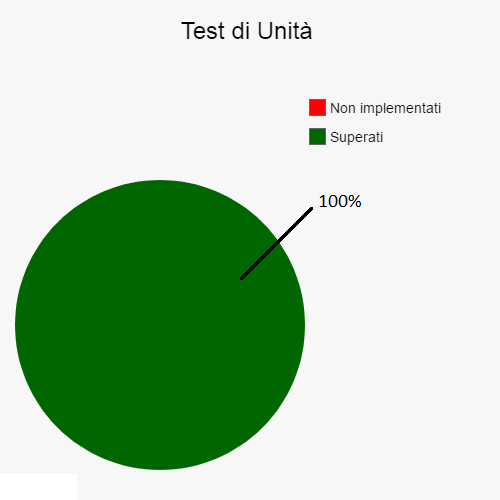
\includegraphics[scale=0.7]{includes/img/test_unita.png}
		\caption{Grado di completamento test di unità}
	\end{figure}
	
	\clearpage
	
	\subsection{Test di integrazione}
	Questa tipologia di test serve a verificare il corretto funzionamento delle singole componenti di sistema progettate durante l'attività di progettazione ad alto livello. Per questa tipologia di test, l'idea è quella di utilizzare un approccio top-down, in modo da sottoporre a test e integrare per primi i moduli di livello più alto.
	Così facendo, però, sarà necessario simulare le componenti di livello inferiore con degli stub. Una volta codificate, le componenti di livello più basso dovranno essere a loro volta integrate e testate.\\
	L'approccio top-down rientra tra le strategie di integrazione incrementale, che consentono di poter determinare in modo più rapido quale componente è la causa di problemi, poichè i difetti rilevati dai test saranno da attribuirsi all'ultima componente aggiunta.
	I test di integrazione saranno descritti nel modo seguente:
	\begin{center}
		\textbf{TI}[\textit{IdComponente}]
	\end{center}
	dove:
	\begin{itemize}
		\item
		\textbf{IdComponente} rappresenta il codice identificativo progressivo del componente preso in considerazione.
	\end{itemize}
	
	% TABELLA
	\normalsize
	\begin{longtable}{|>{\centering\arraybackslash}p{1.5cm}|>{\centering\arraybackslash}p{8cm} | >{\centering\arraybackslash}p{3.8cm}|}
		\hline \rowcolor{Gray}
		\textbf{Id Test} & \textbf{Descrizione} & \textbf{Stato}\\
		\hline
		\endhead
		\hypertarget{TI1}{TI1} & Viene verificato che l’applicazione web \progetto\ gestisca
		correttamente il front-end del prodotto e le sue interazioni con il back-end. & \textcolor{Green}{\textit{Superato}}\\ \hline
		\hypertarget{TI2}{TI2} & Viene verificato che i \textit{Controllers} del front-end si integrino
		correttamente nell’applicazione web. & \textcolor{Green}{\textit{Superato}}\\ \hline
		\hypertarget{TI3}{TI3} & Viene verificato che i \textit{Services} permettano una corretta interazione con il back-end. & \textcolor{Green}{\textit{Superato}}\\ \hline
		\hypertarget{TI4}{TI4} & Viene verificato che il \textit{Model} si integri correttamente con i
		\textit{Services} e con il resto delle componenti dell’applicazione che lo utilizzano. & \textcolor{Green}{\textit{Superato}}\\ \hline
		\hypertarget{TI5}{TI5} & Viene verificato che le \textit{Views} si integrino correttamente con i
		\textit{Controllers}, in modo da visualizzare senza errori i dati ricevuti. & \textcolor{Green}{\textit{Superato}}\\ \hline
		\hypertarget{TI6}{TI6} & Viene verificato che l’applicazione web gestisca	correttamente il back-end del prodotto, in modo tale da fornire al front-end le informazioni richieste. & \textcolor{Green}{\textit{Superato}}\\ \hline
		\hypertarget{TI7}{TI7} & Viene verificato che il \textit{Server} sia configurato e che sia in grado di caricare correttamente tutte le librerie necessarie all'istanziazione delle classi in modo corretto. & \textit{Non implementato}\\ \hline
		\hypertarget{TI8}{TI8} & Viene verificato che la \textit{Single Page App} si integri correttamente con i microservizi \textit{Jolie} utilizzati per il back-end. & \textcolor{Green}{\textit{Superato}}\\ \hline
		\hypertarget{TI9}{TI9} & Viene verificato che i \textit{Controllers} si integrino correttamente
		e gestiscano le richieste inoltrate dai \textit{Routers}. & \textcolor{Green}{\textit{Superato}}\\ \hline
		\hypertarget{TI10}{TI10} & Viene verificato che il \textit{Model} si integri correttamente con i
		\textit{Controllers} per la gestione dell’inserimento, della modifica e della cancellazione dei dati. & \textcolor{Green}{\textit{Superato}}\\ \hline
		\caption[Test di integrazione]{Test di integrazione}
		\label{tabella:test1}
	\end{longtable}

	\subsubsection{Grado di completamento dei test di integrazione}
	Di seguito viene fornito un pie chart che rappresenta il grado di completamento dei \textbf{test di integrazione} implementati e superati.
	\begin{figure}[H]
		\centering
		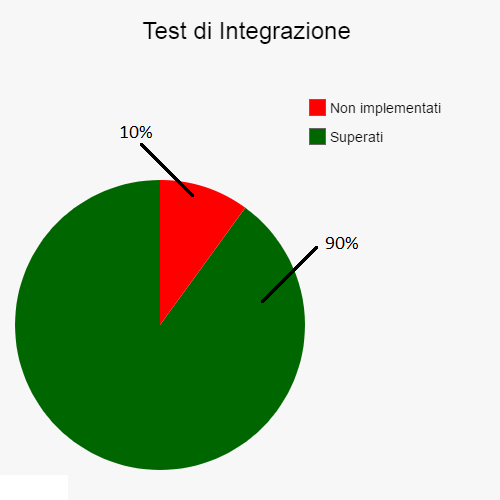
\includegraphics[scale=0.7]{includes/img/test_integrazione.png}
		\caption{Grado di completamento test di integrazione}
	\end{figure}

	\clearpage
	
	\subsection{Test di sistema}
	Questa tipologia di test serve a verificare il corretto comportamento e funzionamento dell’architettura. Tale tipologia di test deve verificare che ci sia la copertura totale dei requisiti software stabiliti durante l'\AdR.
	I test di sistema saranno organizzati nel modo seguente:
	\begin{center}
		\textbf{TS}[\textit{TipologiaRequisito}][\textit{RilevanzaRequisito}][\textit{CodiceRequisito}]
	\end{center}
	dove:
	\begin{itemize}
		\item
		\textbf{TipologiaRequisito} può assumere valori tra:
		\begin{itemize}
			\item
			\textit{V} per i requisiti di vincolo;
			\item
			\textit{F} per i requisiti di funzionalità;
			\item
			\textit{Q} per i requisiti di qualità;
			\item
			\textit{P} per i requisiti prestazionali.
		\end{itemize}
		\item 
		\textbf{RilevanzaRequisito} può assumere valori tra:
		\begin{itemize}
			\item
			\textit{O} per i requisiti obbligatori;
			\item
			\textit{D} per i requisiti desiderabili;
			\item
			\textit{F} per i requisiti facoltativi.
		\end{itemize}
		\item
		\textbf{CodiceRequisito} assume un valore gerarchico che identifica il singolo requisito.
	\end{itemize}
	
	% TABELLA
	\normalsize
	\begin{longtable}{|>{\centering\arraybackslash}p{2.3cm}|>{\centering\arraybackslash}p{7.5cm} | >{\centering\arraybackslash}p{3.8cm}|}
		\hline \rowcolor{Gray}
		\textbf{Id Test} & \textbf{Descrizione} & \textbf{Stato}\\
		\hline
		\endhead
		\hypertarget{TSFO1}{TSFO1} & Viene verificato che il sistema registri correttamente un utente. & \textcolor{Green}{\textit{Superato}}\\ \hline
		\hypertarget{TSFO2}{TSFO2} & Viene verificato che il sistema riesca a far effettuare correttamente il login ad un utente attraverso \progetto. & \textcolor{Green}{\textit{Superato}}\\ \hline	
		\hypertarget{TSFD3}{TSFD3} & Viene verificato che il sistema permetta il recupero della password per un utente registrato ad \progetto. & \textit{Non Implementato}\\ \hline	
		\hypertarget{TSFO4}{TSFO4} & Viene verificato che il sistema ricerchi correttamente una API. & \textcolor{Green}{\textit{Superato}}\\ \hline
		\hypertarget{TSFO4.3}{TSFO4.3} & Viene verificato che il sistema restituisca un insieme di risultati coerenti secondo i parametri di ricerca specificati da un utente. & \textcolor{Green}{\textit{Superato}}\\ \hline	
		\hypertarget{TSFO5}{TSFO5} & Viene verificato che il sistema visualizzi correttamente i dati relativi ad una API. & \textcolor{Green}{\textit{Superato}}\\ \hline
		\hypertarget{TSFO5.6}{TSFO5.6} & Viene verificato che il sistema consenta la consultazione della documentazione di una API. & \textcolor{Green}{\textit{Superato}}\\ \hline
		\hypertarget{TSFO5.7}{TSFO5.7} & Viene verificato che il sistema visualizzi correttamente i dati di utilizzo di una API. & \textit{Non Implementato}\\ \hline
		\hypertarget{TSFO6.2}{TSFO6.2} & Viene verificato che il sistema visualizzi correttamente la lista di API acquistate da un utente. & \textcolor{Green}{\textit{Superato}}\\ \hline
		\hypertarget{TSFO7}{TSFO7} & Viene verificato che il sistema consenta l'acquisto di una API, con conseguente rilascio di una API Key, per un utente. & \textcolor{Green}{\textit{Superato}}\\ \hline
		\hypertarget{TSFO7.5.3}{TSFO7.5.3} & Viene verificato che il sistema crei e visualizzi correttamente l'API Key associata ad una API, per cui è stata acquistata una licenza da un utente. & \textcolor{Green}{\textit{Superato}}\\ \hline
		\hypertarget{TSFO8}{TSFO8} & Viene verificato che il sistema gestisca correttamente le API inserite da uno sviluppatore. & \textcolor{Green}{\textit{Superato}}\\ \hline
		\hypertarget{TSFO8.2}{TSFO8.2} & Viene verificato che il sistema visualizzi correttamente la lista delle API registrate da uno sviluppatore. & \textcolor{Green}{\textit{Superato}}\\ \hline
		\hypertarget{TSFO8.2.4}{TSFO8.2.4} & Viene verificato che il sistema modifichi correttamente le informazioni relative ad una API registrata da uno sviluppatore. & \textcolor{Green}{\textit{Superato}}\\ \hline
		\hypertarget{TSFO8.2.8}{TSFO8.2.8} & Viene verificato che il sistema visualizzi correttamente il guadagno netto, in base alla policy, di una API da lui inserita. & \textit{Non Implementato}\\ \hline
		\hypertarget{TSFO8.2.9}{TSFO8.2.9} & Viene verificato che il sistema elimini correttamente una API su richiesta dello sviluppatore autore. & \textcolor{Green}{\textit{Superato}}\\ \hline
		\hypertarget{TSFO9}{TSFO9} & Viene verificato che il sistema inserisca correttamente nel marketplace una nuova API. & \textcolor{Green}{\textit{Superato}}\\ \hline
		\hypertarget{TSFO10.1}{TSFO10.1} & Viene verificato che il sistema permetta di gestire correttamente ad un utente le informazioni del proprio profilo. & \textcolor{Green}{\textit{Superato}}\\ \hline
		\hypertarget{TSFO10.1.1}{TSFO10.1.1} & Viene verificato che il sistema visualizzi correttamente le informazioni del profilo di un utente. & \textcolor{Green}{\textit{Superato}}\\ \hline
		\hypertarget{TSFO10.1.2}{TSFO10.1.2} & Viene verificato che il sistema modifichi correttamente le informazioni di un utente. & \textcolor{Green}{\textit{Superato}}\\ \hline
		\hypertarget{TSFD10.1.2.9}{TSFD10.1.2.9} & Viene verificato che il sistema effettui correttamente l'upgrade dell'account di un utente. & \textit{Non Implementato}\\ \hline
		\hypertarget{TSFO10.2}{TSFO10.2} & Viene verificato che il sistema permetta di gestire correttamente ad un utente il proprio conto. & \textcolor{Green}{\textit{Superato}}\\ \hline
		\hypertarget{TSFO10.2.1}{TSFO10.2.1} & Viene verificato che il sistema visualizzi correttamente il saldo attuale del conto di un utente. & \textcolor{Green}{\textit{Superato}}\\ \hline
		\hypertarget{TSFO10.2.2}{TSFO10.2.2} & Viene verificato che il sistema permetta ad un utente di ricaricare il saldo del proprio conto attraverso PayPal. & \textit{Non Implementato}\\ \hline
		\hypertarget{TSFO10.3}{TSFO10.3} & Viene verificato che il sistema visualizzi correttamente lo storico delle transazioni di un utente. & \textcolor{Green}{\textit{Superato}}\\ \hline
		\hypertarget{TSFO10.3.2}{TSFO10.3.2} & Viene verificato che il sistema visualizzi correttamente la lista delle transazioni concluse di un utente. & \textcolor{Green}{\textit{Superato}}\\ \hline
		\hypertarget{TSFO11}{TSFO11} & Viene verificato che il sistema riesca a far effettuare correttamente il logout ad un utente.  & \textcolor{Green}{\textit{Superato}}\\ \hline
		\hypertarget{TSFO12.1.1.1}{TSFO12.1.1.1} & Viene verificato che il sistema visualizzi correttamente i dati avanzati di una API da parte di un amministratore. & \textit{Non Implementato}\\ \hline
		\hypertarget{TSFO12.1.1.2}{TSFO12.1.1.2} & Viene verificato che il sistema sospenda correttamente una API su richiesta di un amministratore. & \textcolor{Green}{\textit{Superato}}\\ \hline
		\hypertarget{TSFD12.1.1.3}{TSFD12.1.1.3} & Viene verificato che il sistema elimini correttamente una API su richiesta di un amministratore. & \textcolor{Green}{\textit{Superato}}\\ \hline
		\hypertarget{TSFO12.2.1.1}{TSFO12.2.1.1} & Viene verificato che il sistema permetta ad un amministratore di sospendere correttamente un utente. & \textcolor{Green}{\textit{Superato}}\\ \hline
		\hypertarget{TSFO12.2.1.2}{TSFO12.2.1.2} & Viene verificato che il sistema permetta ad un amministratore di sospendere correttamente i pagamenti veso un utente. & \textit{Non Implementato}\\ \hline
		\hypertarget{TSFO12.2.1.3}{TSFO12.2.1.3} & Viene verificato che il sistema permetta ad un amministratore di revocare correttamente la sospensione ad un utente sospeso. & \textcolor{Green}{\textit{Superato}}\\ \hline
		\hypertarget{TSFO12.2.1.5}{TSFO12.2.1.5} & Viene verificato che il sistema permetta ad un amministratore di eliminare correttamente un utente. & \textcolor{Green}{\textit{Superato}}\\ \hline		
		\hypertarget{TSVO1}{TSVO1} & Viene verificato che il sistema abbia un'architettura a microservizi. & \textcolor{Green}{\textit{Superato}}\\ \hline
		\hypertarget{TSVO2}{TSVO2} & Viene verificato che il sistema utilizzi il linguaggio \textit{Jolie} per l'API Gateway, il back-end dell'applicazione web e le interfacce dei microservizi. & \textcolor{Green}{\textit{Superato}}\\ \hline
		\hypertarget{TSVO3}{TSVO3} & Viene verificato che il sistema utilizzi il linguaggio di markup \textit{HTML5}, unito a fogli di stile in \textit{CSS3} e linguaggio di scripting \textit{JavaScript}. & \textcolor{Green}{\textit{Superato}}\\ \hline
		\hypertarget{TSVO4}{TSVO4} & Viene verificato che il sistema utilizzi il DBMS di tipo relazionale \textit{MySQL}. & \textcolor{Green}{\textit{Superato}}\\ \hline
		\hypertarget{TSVO5}{TSVO5} & Viene verificato che il sistema funzioni su \textit{Google Chrome} versione 55.0 o superiore & \textcolor{Green}{\textit{Superato}}\\ \hline
		\hypertarget{TSVO6}{TSVO6} & Viene verificato che il sistema funzioni su \textit{Mozilla Firefox} versione 51.0 o superiore & \textcolor{Green}{\textit{Superato}}\\ \hline
		\hypertarget{TSVO7}{TSVO7} & Viene verificato che il sistema funzioni su \textit{Safari} versione 10.0 o superiore & \textcolor{Green}{\textit{Superato}}\\ \hline
		\hypertarget{TSVD8}{TSVD8} & Viene verificato che il sistema funzioni su \textit{Opera} versione 42.0 o superiore & \textcolor{Green}{\textit{Superato}}\\ \hline
		\hypertarget{TSVD9}{TSVD9} & Viene verificato che il sistema funzioni su \textit{Internet Explorer} versione 11.0 o superiore & \textcolor{Green}{\textit{Superato}}\\ \hline
		\hypertarget{TSVO10}{TSVO10} & Viene verificato che il sistema funzioni su \textit{Microsoft Edge} versione 38.0 o superiore & \textcolor{Green}{\textit{Superato}}\\ \hline
		\hypertarget{TSVO11}{TSVO11} & Viene verificato che il sistema funzioni su \textit{Android Browser} versione 5.1 o superiore & \textcolor{Green}{\textit{Superato}}\\ \hline
		\hypertarget{TSVO12}{TSVO12} & Viene verificato che il sistema funzioni su \textit{Safari} per iOS 10 o versioni superiori & \textcolor{Green}{\textit{Superato}}\\ \hline
		\hypertarget{TSVF13}{TSVF13} & Viene verificato che il sistema funzioni su \textit{Google Chrome} per iOS versione 56.0 o superiore & \textit{Non Implementato}\\ \hline
		\hypertarget{TSVD14}{TSVD14} & Viene verificato che il sistema funzioni su \textit{Google Chrome} per Android versione 56.0 o superiore & \textit{Non Implementato}\\ \hline
		\caption[Test di sistema]{Test di sistema}
		\label{tabella:test2}
	\end{longtable}
	
	\subsubsection{Grado di completamento dei test di sistema}
	Di seguito viene fornito un pie chart che rappresenta il grado di completamento dei \textbf{test di sistema} implementati e superati.
	\begin{figure}[H]
		\centering
		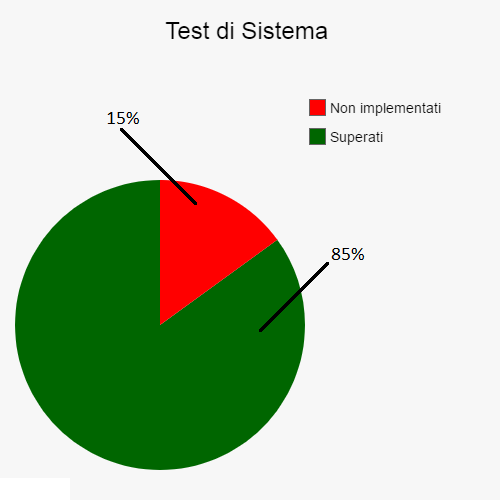
\includegraphics[scale=0.7]{includes/img/test_sistema.png}
		\caption{Grado di completamento test di sistema}
	\end{figure}	
	
	\clearpage
	
	\subsection{Test di non regressione}
	Questa tipologia di test consiste nell'eseguire nuovamente i test che coinvolgono le componenti software che hanno subito modifiche, in modo da verificare che i cambiamenti apportati non compromettano il funzionamento di componenti che non sono stati aggiornati e che, precedentemente, non erano soggetti ad errori.\\
	I test di non regressione saranno descritti nel modo seguente:
	\begin{center}
		\textbf{TNR}[\textit{IdTest}]
	\end{center}
	dove \textbf{\textit{IdTest}} rappresenta il codice identificativo progressivo della modifica apportata, la quale ha prodotto il corrispondente test di non regressione.
	
	% TABELLA
	\normalsize
	\begin{longtable}{|>{\centering\arraybackslash}p{1.5cm}|>{\centering\arraybackslash}p{8cm} | >{\centering\arraybackslash}p{3.8cm}|}
		\hline \rowcolor{Gray}
		\textbf{Id Test} & \textbf{Descrizione} & \textbf{Stato}\\
		\hline
		\endhead
		\hypertarget{TNR1}{TNR1} & Descrizione... & \textcolor{Green}{\textit{Superato}}\\ \hline
		\hypertarget{TNR2}{TNR2} & Descrizione... & \textcolor{Green}{\textit{Superato}}\\ \hline
		\hypertarget{TNR3}{TNR3} & Descrizione... & \textcolor{Green}{\textit{Superato}}\\ \hline
		\hypertarget{TNR4}{TNR4} & Descrizione... & \textcolor{Green}{\textit{Superato}}\\ \hline
		\caption[Test di non regressione]{Test di non regressione}
		\label{tabella:test3}
	\end{longtable}
	
	\subsubsection{Grado di completamento dei test di non regressione}
	Di seguito viene fornito un pie chart che rappresenta il grado di completamento dei \textbf{test di non regressione} implementati e superati.
	\begin{figure}[H]
		\centering
		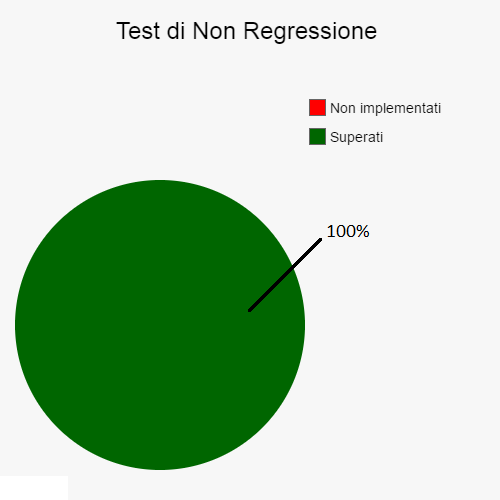
\includegraphics[scale=0.7]{includes/img/test_non_regressione.png}
		\caption{Grado di completamento test di non regressione}
	\end{figure}	
	
	\clearpage
	
	\subsection{Test di validazione}
	Questa tipologia di test serve a verificare che il prodotto soddisfi le richieste del proponente attraverso le funzionalità implementate.\\
	Per questo motivo, occorrerà simulare il comportamento generale dell'applicativo e dell'utente che interagisce con esso, attraverso delle macro azioni.\\
	I test di validazione saranno organizzati nel modo seguente:
	\begin{center}
		\textbf{TV}[\textit{TipologiaRequisito}][\textit{RilevanzaRequisito}][\textit{CodiceRequisito}]
	\end{center}
	dove:
	\begin{itemize}
		\item
		\textbf{TipologiaRequisito} può assumere valori tra:
		\begin{itemize}
			\item
			\textit{V} per i requisiti di vincolo;
			\item
			\textit{F} per i requisiti di funzionalità;
			\item
			\textit{Q} per i requisiti di qualità;
			\item
			\textit{P} per i requisiti prestazionali.
		\end{itemize}
		\item 
		\textbf{RilevanzaRequisito} può assumere valori tra:
		\begin{itemize}
			\item
			\textit{O} per i requisiti obbligatori;
			\item
			\textit{D} per i requisiti desiderabili;
			\item
			\textit{F} per i requisiti facoltativi.
		\end{itemize}
		\item
		\textbf{CodiceRequisito} assume un valore gerarchico che identifica il singolo requisito.
	\end{itemize}

	% TABELLA
	\normalsize
	\begin{longtable}{|>{\centering\arraybackslash}p{2.3cm}|>{\centering\arraybackslash}p{7.5cm} | >{\centering\arraybackslash}p{4cm}|}
		\hline \rowcolor{Gray}
		\textbf{Id Test} & \textbf{Descrizione} & \textbf{Stato}\\
		\hline
		\endhead
		\hypertarget{TVFO1}{TVFO1} & L’utente intende registrarsi alla piattaforma \progetto. All’utente è richiesto di:
		\begin{itemize}
			\item Trovarsi nella sezione apposita;
			\item Compilare il form di registrazione;
			\item Premere il pulsante di conferma;
			\item Verificare attraverso l’autenticazione che la registrazione sia avvenuta correttamente.
		\end{itemize}
		& \textcolor{Green}{\textit{Superato}}\\ \hline
		\hypertarget{TVFO2}{TVFO2} & L’utente intende autenticarsi alla piattaforma \progetto. All’utente è richiesto di:
		\begin{itemize}
			\item Trovarsi nella sezione apposita;
			\item Essere in possesso delle credenziali richieste;
			\item Inserire le credenziali nell’apposito form;
			\item Premere il pulsante di autenticazione;
			\item Verificare che l’autenticazione sia effettivamente avvenuta.
		\end{itemize}
		& \textcolor{Green}{\textit{Superato}}\\ \hline
		\hypertarget{TVFO4}{TVFO4} & L’utente autenticato  intende ricercare una API sul marketplace. All’utente è richiesto di:
		\begin{itemize}
			\item Trovarsi nella sezione apposita;
			\item Ricercare una API digitando le keywords;
			\item Visualizzazione dei risultati della ricerca, secondo le keywords specificate.
		\end{itemize} & \textcolor{Green}{\textit{Superato}}\\ \hline
		\hypertarget{TVFO5}{TVFO5} & L’utente autenticato  intende visualizzare le informazioni relative ad una API. All’utente è richiesto di:
		\begin{itemize}
			\item Trovarsi nella sezione apposita;
			\item Selezionare l'API di cui vuole visualizzare le informazioni;
			\item Visualizzazione dei dati relativi alla API selezionata.
		\end{itemize} & \textcolor{Green}{\textit{Superato}}\\ \hline
		\hypertarget{TVFO5.6}{TVFO5.6} & L’utente autenticato  intende consultare la documentazione relativa ad una API. All’utente è richiesto di:
		\begin{itemize}
			\item Trovarsi nella sezione apposita;
			\item Selezionare l'API di interesse;
			\item Visualizzazione della documentazione dell'API.
		\end{itemize} & \textcolor{Green}{\textit{Superato}}\\ \hline
		\hypertarget{TVFO7}{TVFO7} & L’utente autenticato intende acquistare l'API che sta visualizzando. All’utente è richiesto di:
		\begin{itemize}
			\item Essere autenticato;
			\item Trovarsi nella sezione apposita;
			\item Selezionare la policy di vendita;
			\item Confermare l'acquisto attraverso l'apposito pulsante;
			\item Verificare la transazione nel proprio storico.
		\end{itemize} & \textcolor{Green}{\textit{Superato}}\\ \hline
		\hypertarget{TVFO8.2}{TVFO8.2} & L’utente sviluppatore intende visualizzare l'elenco di API da lui caricate sulla piattaforma \progetto. All’utente è richiesto di:
		\begin{itemize}
			\item Essere autenticato;
			\item Trovarsi nella sezione apposita;
			\item Verificare che vengano visualizzati tutte le proprie API inserite.
		\end{itemize} & \textcolor{Green}{\textit{Superato}}\\ \hline
		\hypertarget{TVFO8.2.3}{TVFO8.2.3} & L’utente sviluppatore intende visualizzare il numero di licenze attive per le API da lui caricate sulla piattaforma \progetto. All’utente è richiesto di:
		\begin{itemize}
			\item Essere autenticato;
			\item Trovarsi nella sezione apposita;
			\item Selezionare una API dall'elenco visualizzato;
			\item Verificare che vengao il numero di licenze attive per la propria API registrata.
		\end{itemize} & \textcolor{Green}{\textit{Superato}}\\ \hline
		\hypertarget{TVFO8.2.4}{TVFO8.2.4} & L’utente sviluppatore intende modificare i dati relativi ad una sua API caricata. All’utente è richiesto di:
		\begin{itemize}
			\item Essere autenticato;
			\item Trovarsi nella sezione apposita;
			\item Premere il pulsante "Modifica API";
			\item Modificare i dati dell'API selezionata;
			\item Premere il pulsante di conferma modifica;
			\item Verificare che sia stata modificata l'API.
		\end{itemize} & \textcolor{Green}{\textit{Superato}}\\ \hline
		\hypertarget{TVFO9}{TVFO9} & L’utente sviluppatore intende caricare una propria API sulla piattaforma \progetto. All’utente è richiesto di:
		\begin{itemize}
			\item Essere autenticato;
			\item Trovarsi nella sezione apposita;
			\item Premere il pulsante "Inserisci API";
			\item Inserire i dati necessari alla pubblicazione della propria API;
			\item Premere il pulsante di conferma inserimento nuova API;
			\item Verificare che sia stata aggiunta al marketplace l'API.
		\end{itemize} & \textcolor{Green}{\textit{Superato}}\\ \hline
		\hypertarget{TVFO10.1.1}{TVFO10.1.1} & L’utente autenticato intende visualizzare il proprio profilo. All’utente è richiesto di:
		\begin{itemize}
			\item Essere autenticato;
			\item Trovarsi nella sezione apposita;
			\item Visualizzare il proprio profilo.
		\end{itemize} & \textcolor{Green}{\textit{Superato}}\\ \hline
		\hypertarget{TVFO10.1.2}{TVFO10.1.2} & L’utente autenticato intende modificare i propri dati. All’utente è richiesto di:
		\begin{itemize}
			\item Essere autenticato;
			\item Trovarsi nella sezione apposita;
			\item Modificare i campi dati consentiti;
			\item Premere il tasto "Conferma Modifiche";
			\item Visualizzare il profilo dell’utente modificato.
		\end{itemize}
		& \textcolor{Green}{\textit{Superato}}\\ \hline
		\hypertarget{TVFD10.1.2.9}{TVFD10.1.2.9} & L’utente autenticato  intende modificare la tipologia di utenza, effettuando un upgrade dell'account. All’utente è richiesto di:
		\begin{itemize}
			\item Essere autenticato;
			\item Trovarsi nella sezione apposita;
			\item Effettuare l'upgrade dell'account, passando da "cliente" a "sviluppatore";
			\item Verificare la modifica effettuata.
		\end{itemize} & \textcolor{Green}{\textit{Superato}}\\ \hline
		\hypertarget{TVFO10.2.1}{TVFO10.2.1} & L’utente intende visualizzare il saldo del proprio conto associato all'account. All’utente è richiesto di:
		\begin{itemize}
			\item Essere autenticato;
			\item Trovarsi nella sezione apposita;
			\item Premere il pulsante "Conto Virtuale";
			\item Visualizzazione del saldo attuale del proprio conto.
		\end{itemize} & \textcolor{Green}{\textit{Superato}}\\ \hline
		\hypertarget{TVFO10.3}{TVFO10.3} & L’utente autenticato intende visualizzare lo storico delle transazioni effettuate. All’utente è richiesto di:
		\begin{itemize}
			\item Essere autenticato;
			\item Trovarsi nella sezione apposita;
			\item Visualizzare lo storico delle transazioni.
		\end{itemize} & \textcolor{Green}{\textit{Superato}}\\ \hline		
		\hypertarget{TVFO11}{TVFO11} & L’utente intende disconnettersi dalla piattaforma \progetto. All’utente è richiesto di:
		\begin{itemize}
			\item Essere autenticato;
			\item Trovarsi nella sezione apposita;
			\item Premere il pulsante di logout;
			\item Verificare che la disconnessione sia effettivamente avvenuta.
		\end{itemize}
		& \textcolor{Green}{\textit{Superato}}\\ \hline
		\hypertarget{TVFO12.2.1}{TVFO12.2.1} & L’utente amministratore della piattaforma \progetto\ intende moderare un determinato utente registrato. All’utente è richiesto di:
		\begin{itemize}
			\item Essere autenticato;
			\item Trovarsi nella sezione apposita;
			\item Selezionare l'utente che si vuole moderare;
			\item Inserire i dati del rapporto di moderazione;
			\item Verificare che l'utente sia stato effettivamente moderato.
		\end{itemize} & \textcolor{Green}{\textit{Superato}}\\ \hline
		\caption[Test di validazione]{Test di validazione}
		\label{tabella:test4}
	\end{longtable}

	\subsubsection{Grado di completamento dei test di validazione}
	Di seguito viene fornito un pie chart che rappresenta il grado di completamento dei \textbf{test di validazione} implementati e superati.
	\begin{figure}[H]
		\centering
		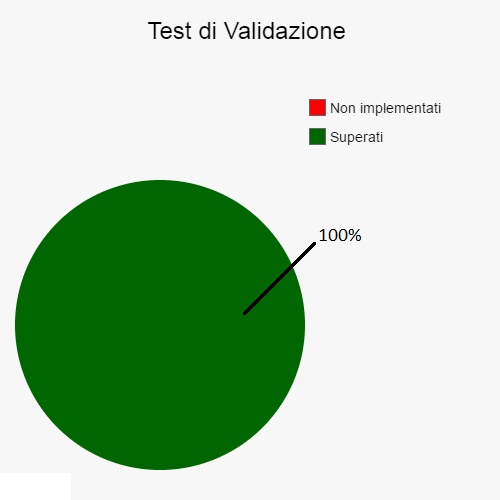
\includegraphics[scale=0.7]{includes/img/test_validazione.png}
		\caption{Grado di completamento test di validazione}
	\end{figure}
	
	\clearpage
	
\newpage
\section{Tracciamento}

\subsection{Tracciamento Test di Unità - Metodi}

% TABELLA
\normalsize
\begin{longtable}{|>{\centering}m{5cm}|m{5cm}<{\centering}|}
	\hline \rowcolor{Gray}
	\textbf{Test} & \textbf{Metodi}\\
	\hline
	\endhead
	
	\caption[Tracciamento Test di Unità-Metodi]{Tracciamento Test di Unità-Metodi}
	\label{tabella:tu-metodi}
\end{longtable}
\clearpage

\subsection{Tracciamento Metodi - Test di Unità}

% TABELLA
\normalsize
\begin{longtable}{|>{\centering}m{5cm}|m{5cm}<{\centering}|}
	\hline \rowcolor{Gray}
	\textbf{Metodi} & \textbf{Test}\\
	\hline
	\endhead
	
	\caption[Tracciamento Metodi-Test di Unità]{Tracciamento Metodi-Test di Unità}
	\label{tabella:metodi-tu}
\end{longtable}
\clearpage

\subsection{Tracciamento Test di Integrazione - Componenti}

% TABELLA
\normalsize
\begin{longtable}{|>{\centering}m{5cm}|m{7cm}<{\centering}|}
	\hline \rowcolor{Gray}
	\textbf{Test} & \textbf{Componenti}\\
	\hline
	\endhead
	\hyperlink{TI1}{TI1} & APIM::FrontEnd::Index \\ \hline
	\hyperlink{TI2}{TI2} & APIM::FrontEnd::App::Controllers \\ \hline
	\hyperlink{TI3}{TI3} & APIM::BackEnd::Services \\ \hline
	\hyperlink{TI4}{TI4} & APIM::FrontEnd::App::Models\\&APIM::BackEnd::Services \\ \hline
	\hyperlink{TI5}{TI5} & APIM::FrontEnd::App::Views\\&APIM::FrontEnd::Controllers \\ \hline
	\hyperlink{TI6}{TI6} & APIM::BackEnd::Services \\ \hline
	\hyperlink{TI7}{TI7} & APIM::FrontEnd::node\_modules\\&APIM::FrontEnd::App::AppRun \\ \hline
	\hyperlink{TI8}{TI8} & APIM::FrontEnd::App::AppRouter\\&APIM::BackEnd::Services\\&APIM::BackEnd::Gateway \\ \hline
	\hyperlink{TI9}{TI9} & APIM::FrontEnd::App::Controllers \\ \hline
	\hyperlink{TI10}{TI10} & APIM::FrontEnd::App::Models\\&APIM::FrontEnd::App::Controllers \\ \hline
	
	\caption[Tracciamento Test di Integrazione-Componenti]{Tracciamento Test di Integrazione-Componenti}
	\label{tabella:ti-componenti}
\end{longtable}
\clearpage

\subsection{Tracciamento Componenti - Test di Integrazione}

% TABELLA
\normalsize
\begin{longtable}{|>{\centering}m{5cm}|m{5cm}<{\centering}|}
	\hline \rowcolor{Gray}
	\textbf{Componenti} & \textbf{Test}\\
	\hline
	\endhead
	
	\caption[Tracciamento Componenti-Test di Integrazione]{Tracciamento Componenti-Test di Integrazione}
	\label{tabella:componenti-ti}
\end{longtable}
\clearpage

\subsection{Tracciamento Test di Sistema - Requisiti}

% TABELLA
\normalsize
\begin{longtable}{|>{\centering}m{5cm}|m{5cm}<{\centering}|}
	\hline \rowcolor{Gray}
	\textbf{Test} & \textbf{Requisito}\\
	\hline
	\endhead
	\hyperlink{TSFO1}{TSFO1} & RFO1\\ \hline
	\hyperlink{TSFO2}{TSFO2} & RFO2\\ \hline
	\hyperlink{TSFD3}{TSFD3} & RFD3\\ \hline
	\hyperlink{TSFO4}{TSFO4} & RFO4\\ \hline
	\hyperlink{TSFO4.3}{TSFO4.3} & RFO4.3\\ \hline
	\hyperlink{TSFO5}{TSFO5} & RFO5\\ \hline
	\hyperlink{TSFO5.6}{TSFO5.6} & RFO5.6\\ \hline
	\hyperlink{TSFO5.7}{TSFO5.7} & RFO5.7\\ \hline
	\hyperlink{TSFO6.2}{TSFO6.2} & RFO6.2\\ \hline
	\hyperlink{TSFO7}{TSFO7} & RFO7\\ \hline
	\hyperlink{TSFO7.5.3}{TSFO7.5.3} & RFO7.5.3\\ \hline
	\hyperlink{TSFO8}{TSFO8} & RFO8\\ \hline
	\hyperlink{TSFO8.2}{TSFO8.2} & RFO8.2\\ \hline
	\hyperlink{TSFO8.2.4}{TSFO8.2.4} & RFO8.2.4\\ \hline
	\hyperlink{TSFO8.2.8}{TSFO8.2.8} & RFO8.2.8\\ \hline
	\hyperlink{TSFO8.2.9}{TSFO8.2.9} & RFO8.2.9\\ \hline
	\hyperlink{TSFO9}{TSFO9} & RFO9\\ \hline
	\hyperlink{TSFO10.1}{TSFO10.1} & RFO10.1\\ \hline
	\hyperlink{TSFO10.1.1}{TSFO10.1.1} & RFO10.1.1\\ \hline
	\hyperlink{TSFO10.1.2}{TSFO10.1.2} & RFO10.1.2\\ \hline
	\hyperlink{TSFD10.1.2.9}{TSFD10.1.2.9} & RFD10.1.2.9\\ \hline
	\hyperlink{TSFO10.2}{TSFO10.2} & RFO10.2\\ \hline
	\hyperlink{TSFO10.2.1}{TSFO10.2.1} & RFO10.2.1\\ \hline
	\hyperlink{TSFO10.2.2}{TSFO10.2.2} & RFO10.2.2\\ \hline
	\hyperlink{TSFO10.3}{TSFO10.3} & RFO10.3\\ \hline
	\hyperlink{TSFO10.3.2}{TSFO10.3.2} & RFO10.3.2\\ \hline
	\hyperlink{TSFO11}{TSFO11} & RFO11\\ \hline
	\hyperlink{TSFO12.1.1.1}{TSFO12.1.1.1} & RFO12.1.1.1\\ \hline
	\hyperlink{TSFO12.1.1.2}{TSFO12.1.1.2} & RFO12.1.1.2\\ \hline
	\hyperlink{TSFD12.1.1.3}{TSFD12.1.1.3} & RFD12.1.1.3\\ \hline
	\hyperlink{TSFO12.2.1.1}{TSFO12.2.1.1} & RFO12.2.1.1\\ \hline
	\hyperlink{TSFO12.2.1.2}{TSFO12.2.1.2} & RFO12.2.1.2\\ \hline
	\hyperlink{TSFO12.2.1.3}{TSFO12.2.1.3} & RFO12.2.1.3\\ \hline
	\hyperlink{TSFO12.2.1.5}{TSFO12.2.1.5} & RFO12.2.1.5\\ \hline
	\hyperlink{TSVO1}{TSVO1} & RVO1\\ \hline
	\hyperlink{TSVO2}{TSVO2} & RVO2\\ \hline
	\hyperlink{TSVO3}{TSVO3} & RVO3\\ \hline
	\hyperlink{TSVO4}{TSVO4} & RVO4\\ \hline
	\hyperlink{TSVO5}{TSVO5} & RVO5\\ \hline
	\hyperlink{TSVO6}{TSVO6} & RVO6\\ \hline
	\hyperlink{TSVO7}{TSVO7} & RVO7\\ \hline
	\hyperlink{TSVD8}{TSVD8} & RVD8\\ \hline
	\hyperlink{TSVD9}{TSVD9} & RVD9\\ \hline
	\hyperlink{TSVO10}{TSVO10} & RVO10\\ \hline
	\hyperlink{TSVO11}{TSVO11} & RVO11\\ \hline
	\hyperlink{TSVO12}{TSVO12} & RVO12\\ \hline
	\hyperlink{TSVF13}{TSVF13} & RVF13\\ \hline
	\hyperlink{TSVD14}{TSVD14} & RVD14\\ \hline	
	\caption[Tracciamento Test di Sistema-Requisiti]{Tracciamento Test di Sistema-Requisiti}
	\label{tabella:ts-requi}
\end{longtable}
\clearpage

\subsection{Tracciamento Requisiti - Test di Sistema}

% TABELLA
\normalsize
\begin{longtable}{|>{\centering}m{5cm}|m{5cm}<{\centering}|}
	\hline \rowcolor{Gray}
	\textbf{Requisito} & \textbf{Test}\\
	\hline
	\endhead

	\caption[Tracciamento Requisiti-Test di Sistema]{Tracciamento Requisiti-Test di Sistema}
	\label{tabella:requi-ts}
\end{longtable}
\clearpage

\subsection{Tracciamento Test di Validazione - Requisiti}

% TABELLA
\normalsize
\begin{longtable}{|>{\centering}m{5cm}|m{5cm}<{\centering}|}
	\hline \rowcolor{Gray}
	\textbf{Test} & \textbf{Requisito}\\
	\hline
	\endhead
	\hyperlink{TVFO1}{TVFO1} & RFO1\\ \hline
	\hyperlink{TVFO2}{TVFO2} & RFO2\\ \hline
	\hyperlink{TVFO4}{TVFO4} & RFO4\\ \hline
	\hyperlink{TVFO5}{TVFO5} & RFO5\\ \hline
	\hyperlink{TVFO5.6}{TVFO5.6} & RFO5.6\\ \hline
	\hyperlink{TVFO7}{TVFO7} & RFO7\\ \hline
	\hyperlink{TVFO8.2}{TVFO8.2} & RFO8.2\\ \hline
	\hyperlink{TVFO8.2.3}{TVFO8.2.3} & RFO8.2.3\\ \hline
	\hyperlink{TVFO8.2.4}{TVFO8.2.4} & RFO8.2.4\\ \hline
	\hyperlink{TVFO9}{TVFO9} & RFO9\\ \hline
	\hyperlink{TVFO10.1.1}{TVFO10.1.1} & RFO10.1.1\\ \hline
	\hyperlink{TVFO10.1.2}{TVFO10.1.2} & RFO10.1.2\\ \hline
	\hyperlink{TVFD10.1.2.9}{TVFD10.1.2.9} & RFO10.1.2.9\\ \hline
	\hyperlink{TVFO10.2.1}{TVFO10.2.1} & RFO10.2.1\\ \hline
	\hyperlink{TVFO10.3}{TVFO10.3} & RFO10.3\\ \hline
	\hyperlink{TVFO11}{TVFO11} & RFO11\\ \hline
	\hyperlink{TVFO12.2.1}{TVFO12.2.1} & RFO12.2.1\\ \hline
	\caption[Tracciamento Test di Validazione-Requisiti]{Tracciamento Test di Validazione-Requisiti}
	\label{tabella:tv-requi}
\end{longtable}
\clearpage